\documentclass[tikz,border=12pt]{standalone}
\usetikzlibrary{calc}
\begin{document}
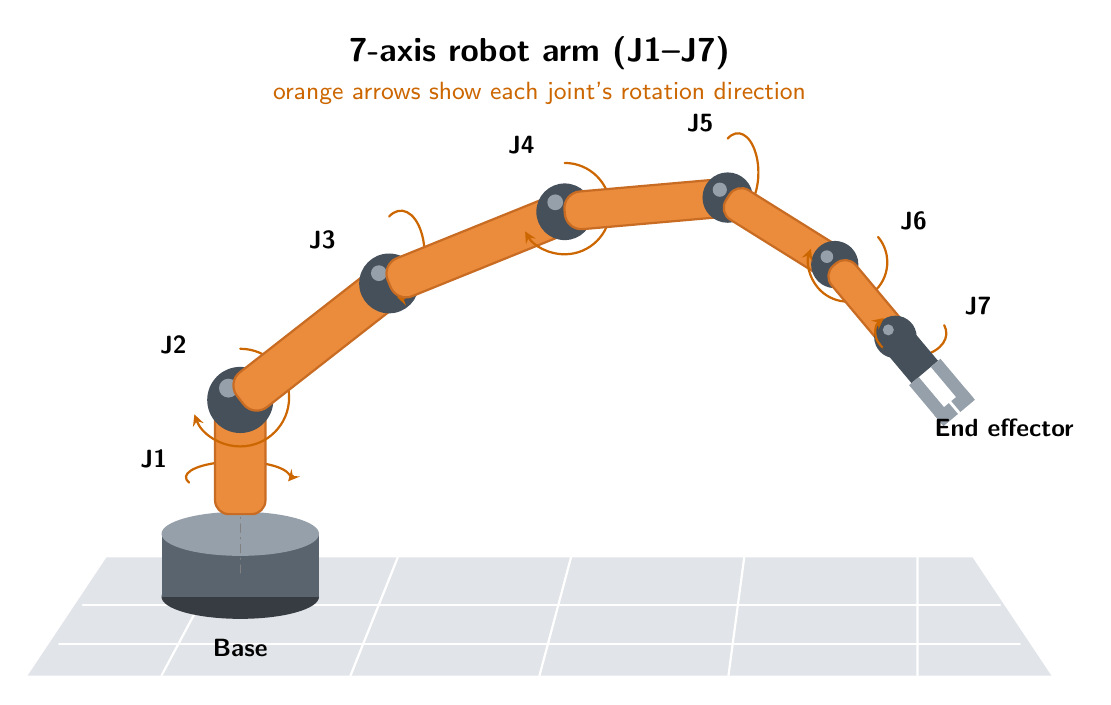
\begin{tikzpicture}[line cap=round,line join=round,>=stealth,
  jlabel/.style={font=\small\sffamily\bfseries,text=black},
  axarrow/.style={->,thick,orange!80!black}]
  \definecolor{basecol}{RGB}{90,100,110}
  \definecolor{linkcol}{RGB}{235,140,60}
  \definecolor{linkdark}{RGB}{200,108,36}
  \definecolor{jointcol}{RGB}{70,80,90}
  \definecolor{jointhi}{RGB}{150,160,170}
  \definecolor{floorcol}{RGB}{225,228,232}

  % floor with light perspective grid
  \fill[floorcol] (-1.5,-0.9) -- (11.5,-0.9) -- (10.5,0.6) -- (-0.5,0.6) -- cycle;
  \draw[white,thick] (0.2,-0.9) -- (1.0,0.6) (2.6,-0.9) -- (3.2,0.6)
    (5.0,-0.9) -- (5.4,0.6) (7.4,-0.9) -- (7.6,0.6) (9.8,-0.9) -- (9.8,0.6);
  \draw[white,thick] (-1.1,-0.5) -- (11.1,-0.5) (-0.8,0.0) -- (10.85,0.0);

  % ---- base (slight 3D cylinder) ----
  \fill[basecol!60!black] (1.2,0.1) ellipse (1.0 and 0.28);
  \fill[basecol] (0.2,0.1) rectangle (2.2,0.9);
  \fill[jointhi] (1.2,0.9) ellipse (1.0 and 0.28);
  \node[jlabel] at (1.2,-0.55) {Base};

  % J1: vertical yaw axis on base
  \draw[gray,dash dot] (1.2,0.4) -- (1.2,2.2);
  \draw[axarrow] (0.55,1.55) arc[start angle=200,end angle=-15,x radius=0.66,y radius=0.2];
  \node[jlabel] at (0.1,1.85) {J1};

  % ---- links and joints ----
  % link1: base to J2
  \fill[linkcol,draw=linkdark,thick,rounded corners=5pt]
    ($(1.2,1.15)+(-0.32,0)$) rectangle ($(1.2,2.6)+(0.32,0)$);
  % J2 (pitch)
  \fill[jointcol] (1.2,2.6) circle (0.42);
  \fill[jointhi] (1.05,2.75) circle (0.12);
  \draw[axarrow] (1.2,3.25) arc[start angle=90,end angle=-160,radius=0.62];
  \node[jlabel] at (0.35,3.3) {J2};

  % link2: J2 to J3
  \fill[linkcol,draw=linkdark,thick,rounded corners=6pt,rotate around={38:(1.2,2.6)}]
    (1.2,2.32) rectangle (3.6,2.88);
  % J3 (roll along link)
  \coordinate (J3) at (3.09,4.08);
  \fill[jointcol] (J3) circle (0.38);
  \fill[jointhi] ($(J3)+(-0.13,0.13)$) circle (0.1);
  \draw[axarrow] ($(J3)+(0.0,0.85)$) arc[start angle=120,end angle=-100,x radius=0.3,y radius=0.55];
  \node[jlabel] at ($(J3)+(-0.85,0.55)$) {J3};

  % link3: J3 to J4
  \fill[linkcol,draw=linkdark,thick,rounded corners=6pt,rotate around={22:(3.09,4.08)}]
    (3.09,3.82) rectangle (5.5,4.34);
  % J4 (pitch)
  \coordinate (J4) at (5.32,4.99);
  \fill[jointcol] (J4) circle (0.36);
  \fill[jointhi] ($(J4)+(-0.12,0.12)$) circle (0.1);
  \draw[axarrow] ($(J4)+(0.0,0.62)$) arc[start angle=90,end angle=-150,radius=0.58];
  \node[jlabel] at ($(J4)+(-0.55,0.85)$) {J4};

  % link4: J4 to J5
  \fill[linkcol,draw=linkdark,thick,rounded corners=6pt,rotate around={5:(5.32,4.99)}]
    (5.32,4.75) rectangle (7.4,5.23);
  % J5 (roll)
  \coordinate (J5) at (7.39,5.17);
  \fill[jointcol] (J5) circle (0.32);
  \fill[jointhi] ($(J5)+(-0.1,0.1)$) circle (0.09);
  \draw[axarrow] ($(J5)+(0.0,0.75)$) arc[start angle=120,end angle=-100,x radius=0.26,y radius=0.5];
  \node[jlabel] at ($(J5)+(-0.35,0.95)$) {J5};

  % link5: J5 to J6 (down toward hand)
  \fill[linkcol,draw=linkdark,thick,rounded corners=5pt,rotate around={-32:(7.39,5.17)}]
    (7.39,4.95) rectangle (9.0,5.39);
  % J6 (pitch)
  \coordinate (J6) at (8.75,4.32);
  \fill[jointcol] (J6) circle (0.3);
  \fill[jointhi] ($(J6)+(-0.1,0.1)$) circle (0.08);
  \draw[axarrow] ($(J6)+(0.55,0.35)$) arc[start angle=40,end angle=-200,radius=0.5];
  \node[jlabel] at ($(J6)+(1.0,0.55)$) {J6};

  % link6: J6 to J7 (wrist)
  \fill[linkcol,draw=linkdark,thick,rounded corners=5pt,rotate around={-50:(8.75,4.32)}]
    (8.75,4.12) rectangle (9.95,4.52);
  % J7 (wrist roll)
  \coordinate (J7) at (9.52,3.4);
  \fill[jointcol] (J7) circle (0.27);
  \fill[jointhi] ($(J7)+(-0.09,0.09)$) circle (0.07);
  \draw[axarrow] ($(J7)+(0.62,0.15)$) arc[start angle=20,end angle=-220,x radius=0.45,y radius=0.3];
  \node[jlabel] at ($(J7)+(1.05,0.4)$) {J7};

  % ---- end effector (gripper) ----
  \begin{scope}[rotate around={-50:(9.52,3.4)}]
    \fill[jointcol] (9.52,3.18) rectangle (10.1,3.62);
    \fill[jointhi] (10.1,3.5) rectangle (10.75,3.66) ;
    \fill[jointhi] (10.1,3.14) rectangle (10.75,3.3);
    \fill[jointhi] (10.6,3.42) rectangle (10.78,3.66);
    \fill[jointhi] (10.6,3.14) rectangle (10.78,3.38);
  \end{scope}
  \node[jlabel] at (10.9,2.25) {End effector};

  % title
  \node[font=\sffamily\bfseries\large] at (5.0,7.0) {7-axis robot arm (J1--J7)};
  \node[font=\small\sffamily,text=orange!80!black] at (5.0,6.5)
    {orange arrows show each joint's rotation direction};
\end{tikzpicture}
\end{document}
